% \clearpage
% Advanced Settings from the \mylib{xparse} Library
\subsection{来自\mylib{xparse}库的高级设置}\label{subsec:sidebyside_xparse}

\begin{marker}

All following macros and options need the \mylib{xparse} library to be
loaded, see \Fullref{sec:xparse}.

所有下面的宏和选项都需要加载 \mylib{xparse}库,见\Fullref{sec:xparse}。

\end{marker}


\begin{docCommand}[doc new=2015-11-20]{tcbsidebyside}{\oarg{options}\marg{left-handed content}\marg{right-handed content}}

Creates a colored box using more or less arbitrary \meta{options} for a \refEnvLe{tcolorbox}.
The \refKeyLe{/tcb/sidebyside} option is set to |true| and the \meta{left-handed content} and \meta{right-handed content} is filled into the box appropriately.
The resulting box is unbreakable.

% 为\refEnvLe{tcolorbox}指定任意的选项\meta{options}创建一个 |tcolorbox| 盒子。%
% \refKeyLe{/tcb/sidebyside}选项被设置为|true|, \meta{left-handed content}和\meta{right-handed content}被适当地填充到盒子中。%
% 这样的盒子是不可分页的。

使用更多或更少任意的\meta{选项}创建一个带有\refEnvLe{tcolorbox}的盒子。
\refKey{/tcb/sidebyside}选项设置为|true|,\meta{左侧内容}和\meta{右侧内容}被适当地填充到盒子中。
生成的盒子不可分割。



\refComLe{tcbsidebyside} is not only a shortcut for using a normal \refEnvLe{tcolorbox} with \refKeyLe{/tcb/sidebyside}, 
but allows setting further options like \refKeyLe{/tcb/sidebyside adapt} and \refKeyLe{/tcb/sidebyside switch}.

% \refComLe{tcbsidebyside}不只是使用普通的\refEnvLe{tcolorbox}指定\refKeyLe{/tcb/sidebyside}的快捷方式, 
% 还允许设置更多的选项,如\refKeyLe{/tcb/sidebyside adapt}和\refKeyLe{/tcb/sidebyside switch}。
\refComLe{tcbsidebyside}不仅是使用普通\refEnvLe{tcolorbox}与\refKeyLe{/tcb/sidebyside}的快捷方式,还允许设置其他选项,如\refKeyLe{/tcb/sidebyside adapt}和\refKeyLe{/tcb/sidebyside switch}。

\begin{dispExample}
% \tcbuselibrary{skins,xparse}
% \usepackage{lipsum}
\tcbsidebyside[title=The Triangle,
  sidebyside adapt=left,
  bicolor,colback=white,colbacklower=yellow!10,
  fonttitle=\bfseries,center title,drop lifted shadow,
]{%
  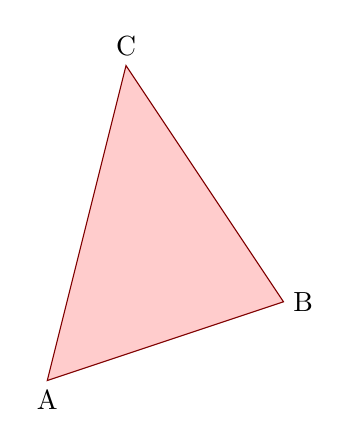
\begin{tikzpicture}
    \path[fill=red!20,draw=red!50!black]
      (0,0) node[below]{A} -- (3,1) node[right]{B}
      -- (1,4) node[above]{C} -- cycle;
  \end{tikzpicture}%
}{%
  \lipsum[1]
}
\end{dispExample}

\begin{dispExample*}{}
\tcbsidebyside[title={sidebyside adapt=left \hfill 左侧变成能不换行的了---virhuiai},
sidebyside adapt=left,
bicolor,colback=white,colbacklower=yellow!10,
fonttitle=\bfseries,center title,drop lifted shadow,
]{农夫倦步长道回家,

仅余我与暮色平分此世界。}{The ploughman

homeward plods his weary way,

And leaves the world

to darkness and to me.
}
\end{dispExample*}
\end{docCommand}